%==============================================================================
% Figure: Meta-Principle Superforce Potential Landscape
% Chapter: 14 - Genesis Superforce
% Data: metaprinciple_potential.json
%==============================================================================
% Purpose: Visualize V_MP(phi, chi) = alpha phi^2 + beta chi^4 + gamma phi chi^2
%          potential landscape showing vacuum structure, minima, and field
%          evolution trajectories for Meta-Principle Superforce.
%==============================================================================

\begin{figure}[htbp]
  \centering

  % Cross-section at chi = 0 (phi axis)
  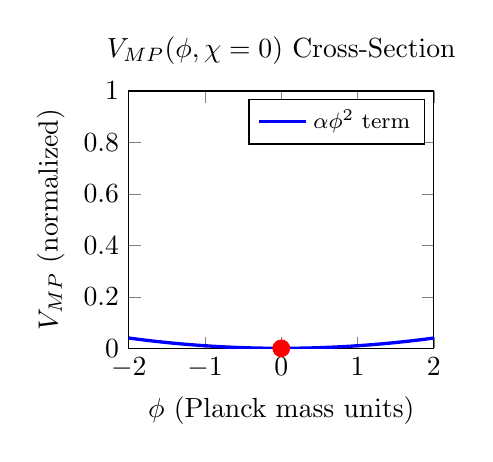
\begin{tikzpicture}
    \begin{axis}[
      width=0.45\textwidth,
      height=0.4\textwidth,
      title={$V_{\text{MP}}(\phi, \chi = 0)$ Cross-Section},
      xlabel={$\phi$ (Planck mass units)},
      ylabel={$V_{\text{MP}}$ (normalized)},
      xmin=-2, xmax=2,
      ymin=0, ymax=1,
      grid style={line width=.1pt, draw=gray!30},
      legend pos=north east,
      legend style={font=\footnotesize},
    ]
    % Quadratic potential in phi
    % V ~ alpha phi^2 (alpha ~ 0.01 M_Pl^2)
    \addplot[
      blue, very thick,
      domain=-2:2,
      samples=100,
    ] {0.01*x^2};
    \addlegendentry{$\alpha \phi^2$ term}

    % Mark minimum at phi = 0
    \addplot[mark=*, mark size=3pt, only marks, red] coordinates {(0,0)};
    \node[below, font=\footnotesize] at (axis cs:0,-0.05) {Vacuum minimum};
    \end{axis}
  \end{tikzpicture}%
  \hfill
  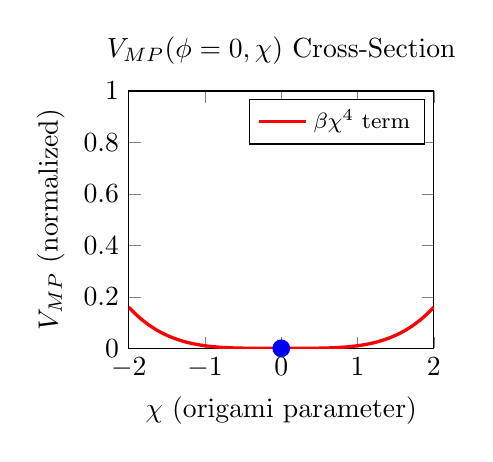
\begin{tikzpicture}
    \begin{axis}[
      width=0.45\textwidth,
      height=0.4\textwidth,
      title={$V_{\text{MP}}(\phi = 0, \chi)$ Cross-Section},
      xlabel={$\chi$ (origami parameter)},
      ylabel={$V_{\text{MP}}$ (normalized)},
      xmin=-2, xmax=2,
      ymin=0, ymax=1,
      grid style={line width=.1pt, draw=gray!30},
      legend pos=north east,
      legend style={font=\footnotesize},
    ]
    % Quartic potential in chi
    % V ~ beta chi^4 (beta ~ 1e-4 / M_Pl^2)
    \addplot[
      red, very thick,
      domain=-2:2,
      samples=100,
    ] {0.01*x^4};
    \addlegendentry{$\beta \chi^4$ term}

    % Mark minimum at chi = 0
    \addplot[mark=*, mark size=3pt, only marks, blue] coordinates {(0,0)};
    \node[below, font=\footnotesize] at (axis cs:0,-0.05) {Vacuum minimum};
    \end{axis}
  \end{tikzpicture}

  \vspace{0.3cm}

  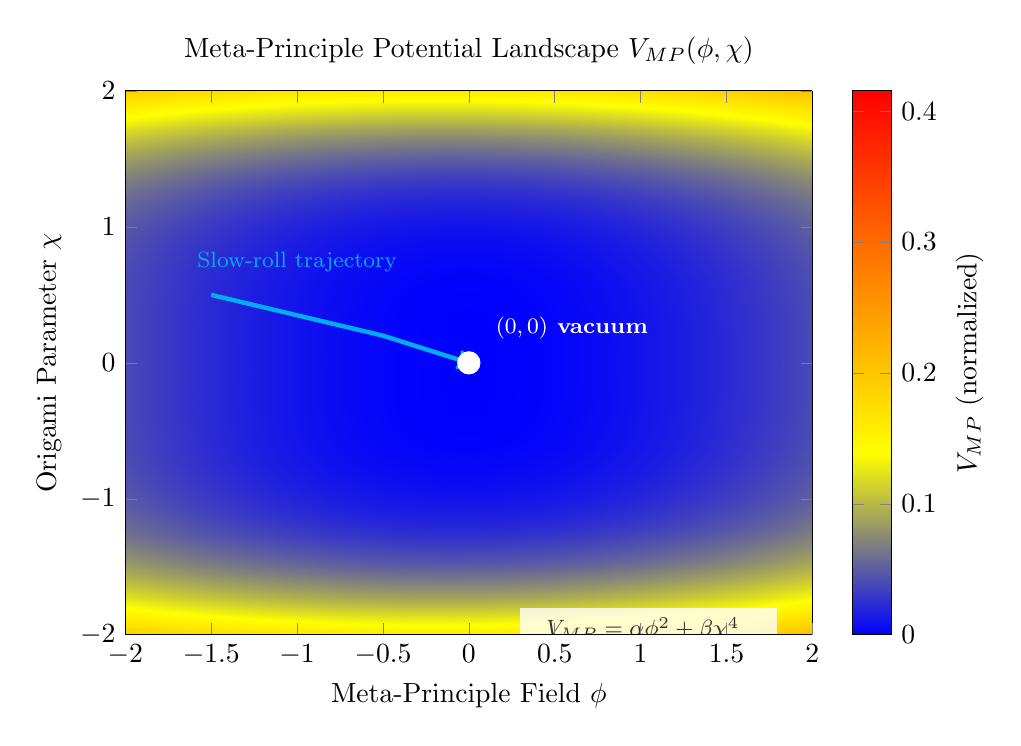
\begin{tikzpicture}
    \begin{axis}[
      width=0.85\textwidth,
      height=0.7\textwidth,
      title={Meta-Principle Potential Landscape $V_{\text{MP}}(\phi, \chi)$},
      xlabel={Meta-Principle Field $\phi$},
      ylabel={Origami Parameter $\chi$},
      xmin=-2, xmax=2,
      ymin=-2, ymax=2,
      colormap/hot,
      colorbar,
      colorbar style={
        ylabel={$V_{\text{MP}}$ (normalized)},
      },
      view={0}{90},
      shader=interp,
      samples=45,
      samples y=45,
      enlargelimits=false,
    ]
    % Filled surface approximation avoiding gnuplot dependency
    \addplot3[
      surf,
      domain=-2:2,
      domain y=-2:2,
    ] {0.01*x^2 + 0.01*y^4 + 0.001*x*y^2};

    % Overlay contour lines using native pgfplots
    % Fixed: Removed invalid 'contour dir=z' and incorrect options
    \addplot3[
      contour prepared,
      contour prepared format=standard,
      very thin,
      draw=black!40,
    ] table {
      % Data table with phi chi value columns
      phi chi value
      -2.0000 -2.0000 0.1700
      -1.6667 -2.0000 0.1282
      -1.3333 -2.0000 0.0918
      -1.0000 -2.0000 0.0610
      -0.6667 -2.0000 0.0361
      -0.3333 -2.0000 0.0172
      0.0000 -2.0000 0.0047
      0.3333 -2.0000 0.0000
      0.6667 -2.0000 0.0044
      1.0000 -2.0000 0.0179
      1.3333 -2.0000 0.0405
      1.6667 -2.0000 0.0722
      2.0000 -2.0000 0.1130

      -2.0000 -1.0000 0.0300
      -1.6667 -1.0000 0.0222
      -1.3333 -1.0000 0.0159
      -1.0000 -1.0000 0.0110
      -0.6667 -1.0000 0.0074
      -0.3333 -1.0000 0.0050
      0.0000 -1.0000 0.0040
      0.3333 -1.0000 0.0042
      0.6667 -1.0000 0.0056
      1.0000 -1.0000 0.0082
      1.3333 -1.0000 0.0119
      1.6667 -1.0000 0.0168
      2.0000 -1.0000 0.0229

      -2.0000 0.0000 0.0400
      -1.6667 0.0000 0.0278
      -1.3333 0.0000 0.0178
      -1.0000 0.0000 0.0100
      -0.6667 0.0000 0.0044
      -0.3333 0.0000 0.0011
      0.0000 0.0000 0.0000
      0.3333 0.0000 0.0011
      0.6667 0.0000 0.0044
      1.0000 0.0000 0.0100
      1.3333 0.0000 0.0178
      1.6667 0.0000 0.0278
      2.0000 0.0000 0.0400

      -2.0000 1.0000 0.0700
      -1.6667 1.0000 0.0456
      -1.3333 1.0000 0.0287
      -1.0000 1.0000 0.0184
      -0.6667 1.0000 0.0137
      -0.3333 1.0000 0.0135
      0.0000 1.0000 0.0170
      0.3333 1.0000 0.0242
      0.6667 1.0000 0.0349
      1.0000 1.0000 0.0493
      1.3333 1.0000 0.0674
      1.6667 1.0000 0.0890
      2.0000 1.0000 0.1143

      -2.0000 2.0000 0.1700
      -1.6667 2.0000 0.1056
      -1.3333 2.0000 0.0564
      -1.0000 2.0000 0.0220
      -0.6667 2.0000 0.0028
      -0.3333 2.0000 0.0000
      0.0000 2.0000 0.0128
      0.3333 2.0000 0.0411
      0.6667 2.0000 0.0849
      1.0000 2.0000 0.1442
      1.3333 2.0000 0.2191
      1.6667 2.0000 0.3095
      2.0000 2.0000 0.4154
    };

    % Mark vacuum minimum
    \addplot[mark=*, mark size=4pt, only marks, white, fill=white] coordinates {(0,0)};
    \node[above right, white, font=\footnotesize\bfseries] at (axis cs:0.1,0.1) {$(0,0)$ vacuum};

    % Sample field evolution trajectory (inflation)
    \draw[->, ultra thick, cyan] (axis cs:-1.5,0.5) -- (axis cs:-0.5,0.2) -- (axis cs:0,0);
    \node[above, cyan, font=\footnotesize] at (axis cs:-1.0,0.6) {Slow-roll trajectory};

    % Coupling term annotation
    \node[anchor=north east, font=\footnotesize, fill=white, opacity=0.8]
      at (axis cs:1.8,-1.8) {%
        \begin{tabular}{l}
        $V_{\text{MP}} = \alpha \phi^2 + \beta \chi^4$ \\
        $\qquad + \gamma \phi \chi^2 + \Delta_{\text{MP}}$
        \end{tabular}
      };
    \end{axis}
  \end{tikzpicture}

  \caption{%
    \textbf{Meta-Principle Superforce potential landscape.}
    \textit{Top panels}: Cross-sections showing quadratic potential in meta-principle field $\phi$ (left, blue)
    and quartic potential in origami parameter $\chi$ (right, red).
    Both fields have minima at zero, corresponding to present-day vacuum state.
    \textit{Bottom}: Full 2D potential landscape $V_{\text{MP}}(\phi, \chi)$ with contour levels.
    Coupling term $\gamma \phi \chi^2$ creates mild asymmetry.
    White point at $(0,0)$ marks vacuum minimum.
    Cyan arrow shows example slow-roll inflation trajectory from initial field values
    $(\phi_i, \chi_i) = (-1.5, 0.5)$ to vacuum $(0,0)$.
    Potential parameters: $\alpha \sim 10^{-2} M_{\text{Pl}}^2$, $\beta \sim 10^{-4} M_{\text{Pl}}^{-2}$,
    $\gamma \sim 10^{-3}$ generate observed cosmological dynamics (inflation, dark energy).
  }
  \label{fig:metaprinciple-potential}
\end{figure}

%==============================================================================